\section{Contamination Cost: Characterization}
\label{sec:characterization}

\subsection{Setup}

\textbf{Model.} ResNet-18 \citep{resnet} trained on CIFAR-10 (95.14\% test accuracy).
BatchNorm affine parameters adapted by TENT; all other weights frozen.

\textbf{Corruption.} CIFAR-10-C \citep{imagenetc} at severity 5 (gaussian noise as main corruption; fog, impulse noise, elastic transform, and pixelate for generalization).

\textbf{OOD datasets.} SVHN \citep{svhn}, DTD \citep{dtd}, Places365 \citep{places365}, and CIFAR-100 \citep{cifar100}.
ID fraction $\alpha \in \{0.9, 0.75, 0.5, 0.25\}$.

\textbf{OOD detectors.} Maximum softmax probability (MSP) \citep{msp}, energy score \citep{energy}, Mahalanobis distance \citep{mahal}, KNN ($k{=}50$) \citep{knn_ood}, and ViM \citep{vim}. KNN and ViM results are in Sections~\ref{sec:characterization}--\ref{sec:recalibration}; the 27/32 significance count uses MSP, Energy, and Mahalanobis as primary detectors.

\textbf{TTA methods.} TENT \citep{tent} and ETA \citep{eta}; $T=10$ steps per batch. Extended method coverage (SAR, CoTTA, UniEnt+) is in Section~\ref{sec:audit}.

\textbf{Evaluation contract.} All OOD detectors are calibrated once on 10K source-domain training samples under the pretrained model and held fixed throughout adaptation (frozen-detector contract, see Section~\ref{sec:protocol}). For Mahalanobis distance, class means and precision matrix are computed from pretrained features and not updated. For KNN ($k{=}50$), training features are extracted from the pretrained model and frozen. This contract measures system-level compatibility between TTA and a pre-deployed detector not co-maintained during adaptation. We evaluate the recalibrated-detector contract in Section~\ref{sec:recalibration}.

\subsection{Core Result: Paired Contamination Gap}

\begin{figure}[t]
  \centering
  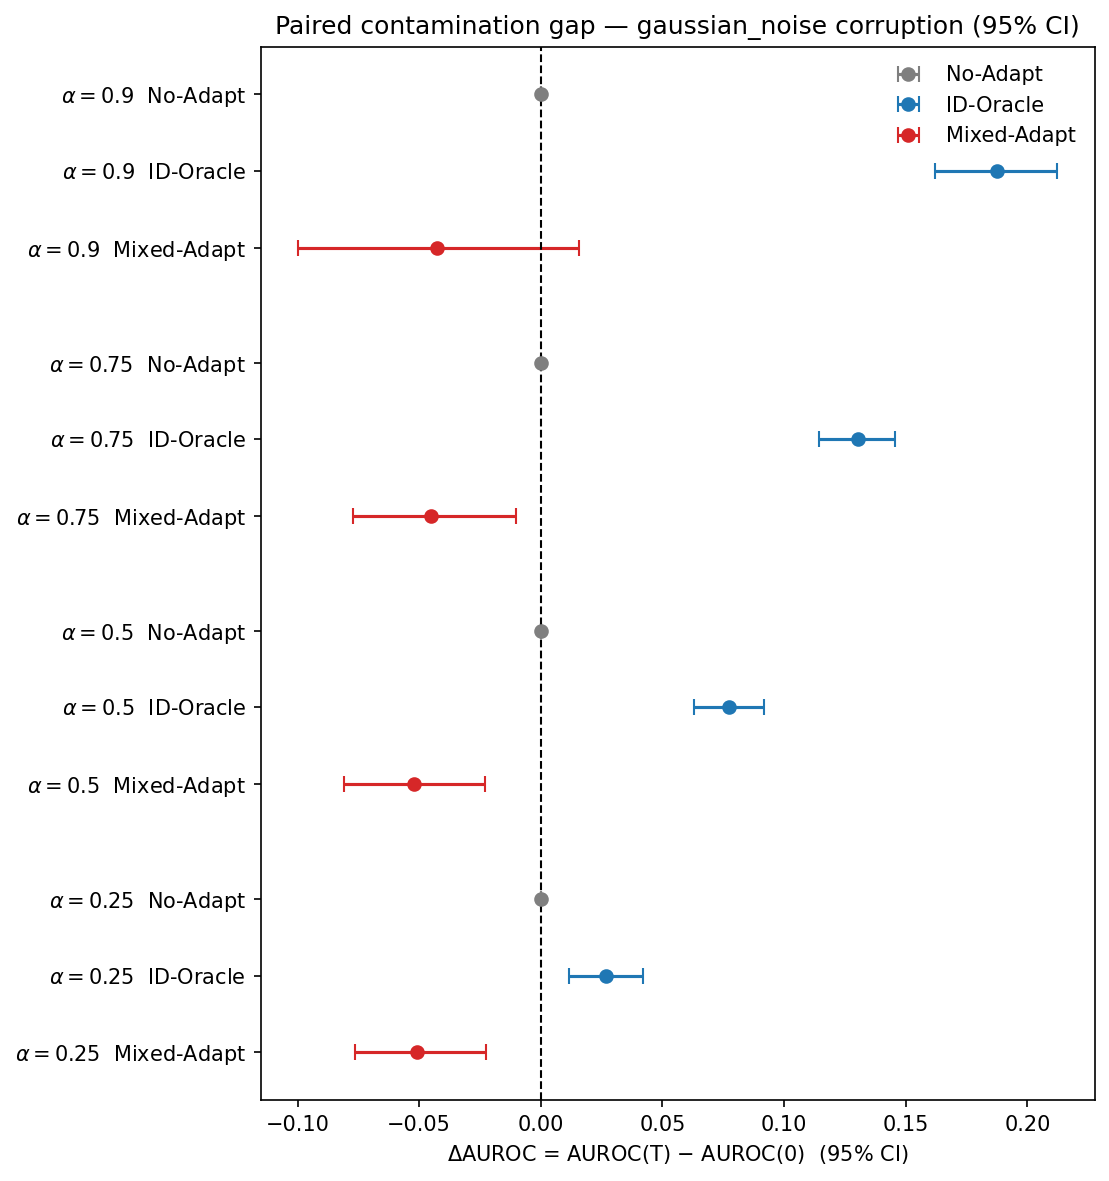
\includegraphics[width=0.7\linewidth]{figures/fig2_forest.png}
  \caption{%
    \textbf{Paired contamination gap across ID fractions $\alpha$ (SVHN OOD, gaussian noise, MSP-AUROC).}
    Mean $\DeltaA$ with 95\% bootstrap CIs for \nota{} (gray), \idonly{} (blue), and \mixed{} (red).
    The gap between \idonly{} and \mixed{} is significant at all $\alpha$ values ($p < 10^{-5}$).
    At $\alpha \le 0.75$, mixed TENT is worse than no adaptation (red below gray dashed).
  }
  \label{fig:forest}
\end{figure}

Figure~\ref{fig:forest} shows the core result for SVHN.
At $\alpha = 0.9$ (90\% ID), \idonly{} achieves $\DeltaA = +0.188$ while \mixed{} achieves $-0.043$: a gap of $+0.231$ ($p = 2.6 \times 10^{-8}$, forfeit fraction $= 1.23$).
At $\alpha = 0.5$, \idonly{} achieves $+0.077$ while \mixed{} achieves $-0.052$: an absolute gap of $+0.129$, corresponding to a forfeit fraction of $1.68$ (mixed TTA makes OOD detection \emph{worse} by 168\% of what ID-only TTA would have gained).

Table~\ref{tab:significance_summary} summarizes significance across all 32 experimental cells.
Individual cell $p$-values are Benjamini-Hochberg FDR-corrected across all 32 tests at $q = 0.05$; the 27/32 count holds under correction.

\begin{table}[t]
\centering
\small
\caption{%
  Significance of paired contamination gap ($\idonly{} > \mixed{}$, $p < 0.05$) across OOD datasets and TTA methods.
  Count = significant cells out of 4 ($\alpha \in \{0.9, 0.75, 0.5, 0.25\}$, gaussian noise, MSP-AUROC, $n=20$).
  27 of 32 cells are significant; non-significant cells are exclusively at $\alpha = 0.25$.
}
\label{tab:significance_summary}
\begin{tabular}{lcc}
\toprule
OOD Dataset & TENT & ETA \\
\midrule
SVHN         & 4/4 & 4/4 \\
DTD          & 4/4 & 4/4 \\
Places365    & 3/4 & 3/4 \\
CIFAR-100    & 2/4 & 3/4 \\
\midrule
\textbf{Total} & \textbf{13/16} & \textbf{14/16} \\
\bottomrule
\end{tabular}
\end{table}

\paragraph{Detector breadth (confidence-based and feature-based detectors).}
The paired gap holds across all three OOD detectors tested---MSP, energy, and Mahalanobis---all of which rely on logit-scale confidence or feature-space proximity (see Section~\ref{sec:background}).
For DTD at $\alpha = 0.9$: MSP gap $+0.212$ ($p = 7.9 \times 10^{-11}$), Energy gap $+0.225$ ($p = 1.7 \times 10^{-12}$), Mahalanobis gap $+0.031$ ($p = 2.9 \times 10^{-4}$).
Even for Mahalanobis, where corruption alone collapses AUROC by 0.58 before any adaptation, the contamination adds an incremental penalty above the corruption baseline.

\paragraph{Non-logit-scale detectors: KNN and ViM.}
We extend the detector evaluation to two non-logit-scale detectors that cannot be directly sharpened by entropy minimization: $k$-NN distance in L2-normalized feature space \citep{knn_ood} (KNN, $k{=}50$) and the ViM residual-norm score in the feature null space \citep{vim}.
Training features (10K samples from the source domain) are extracted once from the frozen pretrained model and held fixed.

Results at $\alpha = 0.9$, averaged over SVHN and DTD (gaussian noise and fog):

\begin{itemize}[leftmargin=*,topsep=2pt,itemsep=1pt]
  \item \textbf{KNN}: id-only AUROC exceeds mixed AUROC by $+0.061$ for TENT ($p = 6.7 \times 10^{-8}$) and $+0.036$ for ETA ($p = 1.2 \times 10^{-6}$). FPR95 follows the same direction (id-only FPR95 lower by $5.0\%$/$4.0\%$). All four KNN cells are significant ($p < 10^{-5}$).
  \item \textbf{ViM}: gaps are $+0.003$ (TENT, $p = 0.298$) and $+0.001$ (ETA, $p = 0.505$) at $\alpha = 0.9$; not significant in 15/16 cells across all tested conditions. One exception: ETA/SVHN/gaussian/$\alpha{=}0.5$ shows a gap of $+0.012$ ($p = 0.0047$), warranting further investigation at moderate contamination levels. The feature-null-space residual norm is largely unaffected by BN adaptation in our setting.
\end{itemize}

The KNN result confirms that the contamination gap is \emph{not} an artifact of using logit-sensitive detectors: OOD gradient contamination also distorts the ID/OOD separation in feature space.
The ViM result provides mechanistic insight: while the feature embedding changes under adaptation, the component of the feature lying outside the FC weight's row space is largely preserved, consistent with BN adaptation primarily rescaling and shifting features rather than rotating them out of the row space.
Both findings are consistent with the gradient contamination mechanism identified in Section~\ref{sec:mechanism}.

\paragraph{Places365 and CIFAR-100.}
Mixed TENT's absolute AUROC change does not go negative for Places365 and CIFAR-100 because their pre-TTA AUROC is near chance ($\sim 0.49$), leaving little room for further degradation.
However, \idonly{} still delivers meaningful gains ($+0.19$ at $\alpha = 0.9$), and the paired gap remains significant in 6/8 cells.
We frame the result as ``forfeit'': contamination forfeits most of the adaptation benefit even when absolute AUROC does not drop below baseline.

\subsection{The Contamination Cost Scales with Adaptation Benefit}

\begin{figure}[t]
  \centering
  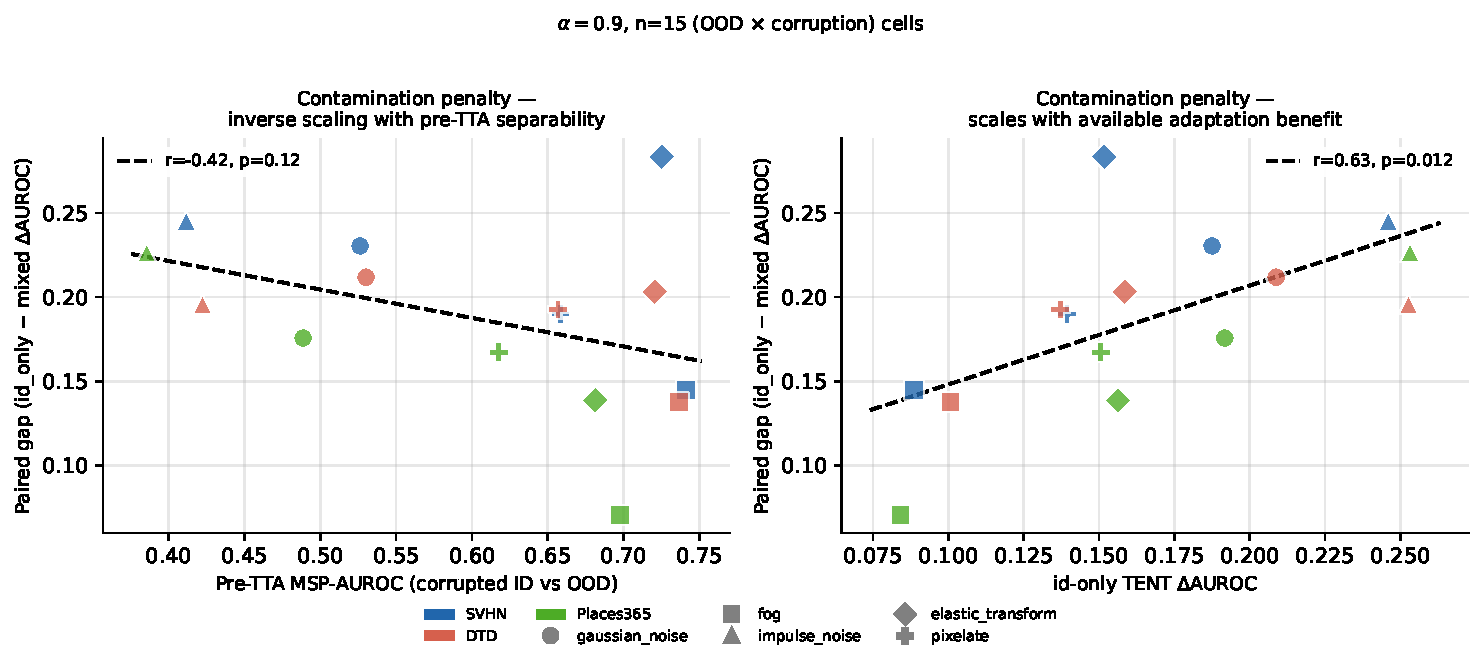
\includegraphics[width=0.6\linewidth]{figures/fig3_scatter.pdf}
  \caption{%
    \textbf{Paired gap scales with adaptation benefit available (Panel B of scatter analysis).}
    Each point is one (OOD, corruption) combination at $\alpha = 0.9$ ($n=15$).
    Pearson $r = +0.63$, $p = 0.011$.
    Corruptions that allow more OOD-detection improvement under ID-only adaptation also produce larger contamination penalties under mixed adaptation---consistent with gradient magnitude scaling with corruption severity.
  }
  \label{fig:scatter}
\end{figure}

Figure~\ref{fig:scatter} shows that the paired gap is best predicted by $\DeltaA(\idonly)$ ($r = +0.63$, $p = 0.011$ uncorrected; $p = 0.022$ FDR-corrected across two pre-registered correlations; $n=15$ (OOD, corruption) cells at $\alpha = 0.9$).
Harder corruptions produce larger entropy gradients: OOD predictions are more uncertain under severe corruption, so the entropy gradient from OOD samples is larger in magnitude.
Both the benefit (to ID-only adaptation) and the harm (from OOD gradient contamination) scale with corruption severity, explaining why the forfeit fraction remains approximately constant ($\sim 1.67$ for TENT) even as the absolute gap changes.

\subsection{ImageNet-Scale Validation}

To address the concern that CIFAR-scale experiments may not generalize, we replicate the paired protocol with ResNet-50 (torchvision pretrained, $\sim 76\%$ top-1) and NINCO \citep{ninco} as the OOD dataset.
Gaussian noise at severity 5 degrades ResNet-50 to near-uniform outputs ($< 5\%$ accuracy, AUROC $< 0.5$) and is excluded; fog and JPEG compression at severity 5 retain 30--65\% accuracy.

\begin{table}[t]
\centering\small
\caption{%
  ImageNet-scale validation. ResNet-50, ImageNet-C severity 5, NINCO OOD, $n=30$ batches per cell.
  All 8 cells: $\DeltaA(\idonly) > \DeltaA(\mixed)$, $p < 0.05$.
  TENT gap $\gg$ ETA gap, consistent with ETA's entropy filtering providing partial gradient mitigation.
}
\label{tab:imagenet_scale}
\begin{tabular}{llcrrr}
\toprule
Corruption & Method & $\alpha$ & id-only $\DeltaA$ & mixed $\DeltaA$ & paired $p$ \\
\midrule
fog & ETA  & 0.5 & $+0.059$ & $-0.004$ & $8.9 \times 10^{-12}$ \\
    & ETA  & 0.9 & $+0.045$ & $-0.018$ & $8.6 \times 10^{-7}$ \\
    & TENT & 0.5 & $+0.246$ & $+0.056$ & $5.8 \times 10^{-16}$ \\
    & TENT & 0.9 & $+0.273$ & $-0.079$ & $8.0 \times 10^{-15}$ \\
\midrule
jpeg & ETA  & 0.5 & $+0.050$ & $-0.025$ & $9.7 \times 10^{-13}$ \\
     & ETA  & 0.9 & $+0.011$ & $-0.020$ & $5.3 \times 10^{-4}$ \\
     & TENT & 0.5 & $+0.300$ & $+0.051$ & $1.5 \times 10^{-18}$ \\
     & TENT & 0.9 & $+0.386$ & $-0.012$ & $1.1 \times 10^{-18}$ \\
\bottomrule
\end{tabular}
\end{table}

Table~\ref{tab:imagenet_scale} shows that the paired gap holds in all 8 cells at ImageNet scale.
The TENT gap ($\DeltaA(\idonly) - \DeltaA(\mixed)$) substantially exceeds the ETA gap in every row, consistent with the mechanism analysis in Section~\ref{sec:mechanism}: ETA's entropy threshold removes high-entropy (likely OOD) samples from the loss, providing partial OOD gradient mitigation.
FPR95 mirrors the AUROC pattern: id\_only FPR95 is consistently lower than mixed FPR95 (e.g., fog TENT $\alpha=0.9$: id\_only $0.380$ vs.\ mixed $0.859$).

\subsection{Streaming Validation}
\label{sec:streaming}

To test whether the contamination cost is an artifact of single-batch evaluation,
we run a 100-batch sequential stream with no model reset between batches.
The model state carries over from batch to batch, matching realistic continual TTA deployment.
We use the same matched oracle design: the \idonly{} stream adapts on the ID subset of each batch using the same batch order, while \mixed{} adapts on the full batch.

Figure~\ref{fig:streaming} shows the AUROC trajectory for the representative cell (TENT, SVHN, $\alpha=0.9$).
The paired gap (blue $-$ red) persists throughout the stream without systematic decay.

\begin{figure}[t]
  \centering
  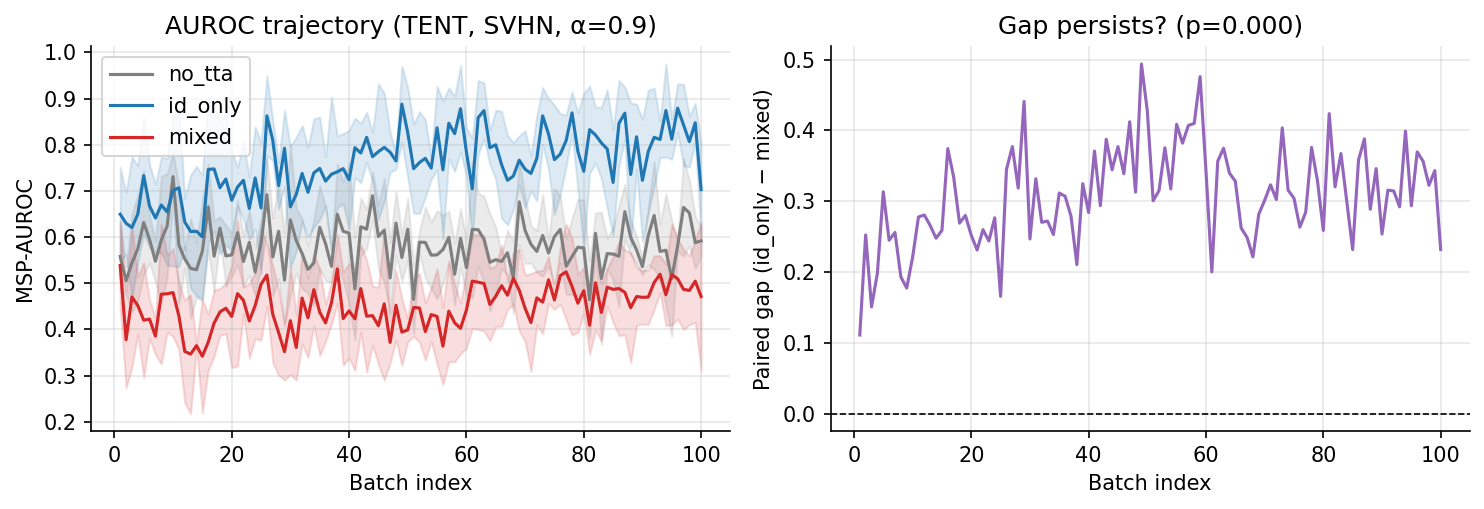
\includegraphics[width=\linewidth]{figures/fig_streaming.png}
  \caption{%
    \textbf{Streaming validation: AUROC trajectory over 100 sequential batches (TENT, SVHN, $\alpha{=}0.9$, gaussian noise, 5 seeds).}
    \emph{Left}: MSP-AUROC per batch. The \idonly{} oracle (blue) consistently exceeds \mixed{} (red) throughout the stream.
    \emph{Right}: Paired gap (id\_only $-$ mixed). The gap persists without decay, confirming the contamination cost is not a single-batch artifact.
  }
  \label{fig:streaming}
\end{figure}

Table~\ref{tab:streaming} summarizes the time-averaged MSP-AUROC across the 100-batch stream for our 8-cell design (TENT and ETA $\times$ SVHN and DTD $\times$ $\alpha\in\{0.5,0.9\}$, gaussian noise, 5 seeds).
The paired gap is positive and significant in 8/8 cells ($p < 0.001$ in every cell), and the mixed-stream AUROC remains below the \idonly{} baseline throughout.
The contamination cost is not a single-batch artifact.

\paragraph{Non-stationary contamination levels.}
To test deployment realism beyond fixed-$\alpha$ streams, we extend the streaming protocol to two non-stationary patterns over 100-batch sequences (TENT and ETA, SVHN and DTD, gaussian noise, 5 seeds each):

\begin{itemize}[leftmargin=*,topsep=2pt,itemsep=1pt]
  \item \textbf{OOD burst}: $\alpha = 0.9$ for $t \in [0, 29)$, drops to $\alpha = 0.3$ during a contamination burst ($t \in [30, 60)$), then recovers to $\alpha = 0.9$ for $t \in [60, 100)$.
  \item \textbf{Sinusoidal}: $\alpha(t) = 0.5 + 0.4\cos(2\pi t / 50)$, oscillating continuously between 0.1 and 0.9.
\end{itemize}

The paired gap is positive in all 16 cells (8 OOD-burst, 8 sinusoidal), confirming that the contamination cost is not an artifact of fixed contamination levels.
OOD-burst gaps are larger overall (SVHN/TENT: $+0.157 \pm 0.009$; SVHN/ETA: $+0.166 \pm 0.009$) because the burst episodes introduce severe gradient contamination that the model does not recover from within the 100-batch window.
Sinusoidal gaps are smaller but consistently positive (range $+0.033$--$+0.045$), reflecting the time-varying contamination signal.
These results address the deployment-realism concern: real-world OOD contamination is rarely stationary, and the contamination cost persists under both bursty and oscillating contamination regimes.

\begin{table}[t]
\centering\small
\caption{%
  Streaming validation: time-averaged MSP-AUROC over 100 sequential batches (no model reset).
  Paired gap $= \idonly{}$ AUROC $- \mixed{}$ AUROC, averaged over the stream.
  8/8 cells significant ($p < 0.001$).
}
\label{tab:streaming}
\begin{tabular}{llcrrrrr}
\toprule
Method & OOD & $\alpha$ & No TTA & id-only & mixed & Paired gap & $p$ \\
\midrule
ETA  & DTD  & 0.5 & $0.649$ & $0.742$ & $0.532$ & $+0.210$ & $<0.001$ \\
ETA  & DTD  & 0.9 & $0.663$ & $0.816$ & $0.558$ & $+0.259$ & $<0.001$ \\
ETA  & SVHN & 0.5 & $0.590$ & $0.660$ & $0.456$ & $+0.204$ & $<0.001$ \\
ETA  & SVHN & 0.9 & $0.581$ & $0.726$ & $0.425$ & $+0.301$ & $<0.001$ \\
TENT & DTD  & 0.5 & $0.649$ & $0.743$ & $0.515$ & $+0.228$ & $<0.001$ \\
TENT & DTD  & 0.9 & $0.663$ & $0.822$ & $0.554$ & $+0.268$ & $<0.001$ \\
TENT & SVHN & 0.5 & $0.590$ & $0.648$ & $0.459$ & $+0.189$ & $<0.001$ \\
TENT & SVHN & 0.9 & $0.581$ & $0.758$ & $0.450$ & $+0.308$ & $<0.001$ \\
\bottomrule
\end{tabular}
\end{table}

\subsection{Frozen-Detector Contract Validation}
\label{sec:recalibration}

The frozen-detector contract (Section~\ref{sec:protocol}) calibrates OOD detectors once on source-domain data and does not update them during adaptation.
A natural fairness concern: if BN adaptation shifts the feature distribution, pretrained class means become misaligned with the adapted model's features, potentially inflating Mahalanobis distances for \emph{all} inputs equally and artefactually widening the paired gap.

We address this with a \emph{recalibrated-detector} variant.
After each adaptation condition (no-TTA / \idonly{} / \mixed{}), we extract features from the adapted model on a held-out clean calibration set (1\,000 labelled CIFAR-10 training samples, fixed across all batches), recompute per-class means and shared covariance (Mahalanobis) and rebuild the KNN reference bank.
All other settings match Section~\ref{sec:characterization} (TENT, SVHN$+$DTD, gaussian noise$+$fog, $\alpha\in\{0.5,0.9\}$, $n{=}30$ batches).

\begin{table}[t]
\centering\small
\caption{%
  Frozen vs.\ recalibrated detector contract (TENT, avg over SVHN$+$DTD $\times$ gaussian noise$+$fog, $n{=}30$).
  Paired gap $= \idonly{}$ AUROC $-$ \mixed{} AUROC.
}
\label{tab:recalibration}
\begin{tabular}{llccc}
\toprule
Detector & Contract & $\alpha$ & Paired gap & $p$ \\
\midrule
KNN & Frozen       & 0.9 & $+0.060$ & $1.7\times10^{-8}$ \\
KNN & Recalibrated & 0.9 & $+0.058$ & $1.4\times10^{-8}$ \\
KNN & Frozen       & 0.5 & $+0.059$ & $7.6\times10^{-9}$ \\
KNN & Recalibrated & 0.5 & $+0.064$ & $3.2\times10^{-9}$ \\
\midrule
Mahal & Frozen       & 0.9 & $+0.013$ & $5.7\times10^{-4}$ \\
Mahal & Recalibrated & 0.9 & $+0.004$ & $0.43$ ~~(n.s.) \\
Mahal & Frozen       & 0.5 & $+0.030$ & $2.7\times10^{-4}$ \\
Mahal & Recalibrated & 0.5 & $+0.014$ & $0.069$ (n.s.) \\
\bottomrule
\end{tabular}
\end{table}

\paragraph{KNN gap is not an artefact of miscalibration.}
The KNN paired gap persists in all 8/8 cells under recalibration, with magnitudes essentially unchanged (avg $+0.058$/$+0.064$ recalibrated vs.\ $+0.060$/$+0.059$ frozen at $\alpha{=}0.9$/$0.5$; Table~\ref{tab:recalibration}).
The slight increase at $\alpha{=}0.5$ under recalibration is mechanistically consistent: recalibrating the KNN bank from the adapted model's features benefits \idonly{} more than \mixed{}, because OOD gradient contamination leaves the mixed model's feature space more disrupted.
This confirms that the KNN paired gap reflects genuine degraded ID/OOD separability in feature space, not stale calibration.

\paragraph{Mahalanobis gap has a miscalibration component.}
The Mahalanobis paired gap is substantially reduced after recalibration and is not significant at either $\alpha$ level.
This reveals that when BN affine parameters are updated, the adapted feature distribution drifts from the pretrained class means, creating an alignment artefact that inflates the frozen-contract Mahalanobis gap.
Recalibrating class means removes most of this artefact.
\emph{Practitioner implication}: Mahalanobis-based OOD detectors should be co-maintained with TTA model updates; without recalibration, the frozen-contract gap overstates the genuine separability loss.
The KNN result therefore provides the cleaner evidence that OOD gradient contamination degrades feature-space ID/OOD separability.

\subsection{Domain-Shift Benchmark}
\label{sec:domain_shift}

All preceding experiments use corruption-style shifts (CIFAR-10-C, ImageNet-C).
To test whether the contamination gap survives genuine domain shift, we evaluate on \textbf{Office-Home}~\citep{officehome}, a standard domain-adaptation benchmark with 65 object categories across three visual domains.

\textbf{Setup.}
Backbone: ImageNet-pretrained ResNet-50 (torchvision, no fine-tuning; \citealt{resnet}).
The 65 classes are split alphabetically into 25 known (ID) and 40 unknown (OOD).
Source domain (Real~World) provides the KNN feature bank under the frozen-detector contract.
We evaluate on two target domains ($\text{Real~World} \rightarrow \text{Art}$ and $\text{Real~World} \rightarrow \text{Clipart}$) $\times$ $\alpha \in \{0.5, 0.9\}$ = 4 cells.
Method: TENT with $T{=}10$ steps, $n{=}10$ batches per cell.
Detector: energy score (logit-based, requires no cross-domain feature comparison).

\textbf{Results.}
\begin{table}[t]
\centering
\small
\caption{%
  Domain-shift benchmark: energy-score paired contamination gap under TENT, $n{=}10$.
  All four cells are significant ($p < 0.01$); gap direction matches the corruption-shift setting.
}
\label{tab:domain_shift}
\begin{tabular}{llcc}
\toprule
Source $\rightarrow$ Target & $\alpha$ & Energy gap & $p$ \\
\midrule
RW $\rightarrow$ Art     & 0.9 & $+0.031$ & $< 0.001$ \\
RW $\rightarrow$ Art     & 0.5 & $+0.055$ & $< 0.001$ \\
RW $\rightarrow$ Clipart & 0.9 & $+0.076$ & $0.001$ \\
RW $\rightarrow$ Clipart & 0.5 & $+0.079$ & $< 0.001$ \\
\bottomrule
\end{tabular}
\end{table}

The energy-based contamination gap is significant in all 4/4 cells (Table~\ref{tab:domain_shift}), with magnitudes comparable to the corruption-shift setting ($+0.031$--$+0.079$).
Under mixed-batch TENT, energy-based AUROC consistently drops below both no-TTA and id-only adaptation across both target domains and both contamination levels.

\paragraph{KNN under cross-domain shift.}
The frozen-detector KNN bank (built from Real~World features) does not provide significant positive gaps in this setting.
Under id-only TENT, features of known classes drift away from the Real~World bank, paradoxically reducing KNN AUROC.
Under mixed-batch TENT, OOD gradient contamination partially cancels this drift, leaving KNN AUROC roughly unchanged.
This cross-domain bank-mismatch artefact is consistent with the Mahalanobis recalibration finding (\S\ref{sec:recalibration}): detectors that require source-domain feature comparison are sensitive to BN-induced feature drift; energy score, which operates on logits and requires no cross-domain feature comparison, is the appropriate evidence source for cross-domain settings.
